\let\negmedspace\undefined
\let\negthickspace\undefined
\documentclass[journal,12pt,onecolumn]{IEEEtran}
\usepackage{cite}
\usepackage{amsmath,amssymb,amsfonts,amsthm}
\usepackage{amsmath}
\usepackage{algorithmic}
\usepackage{graphicx}
\usepackage{textcomp}
\usepackage{xcolor}
\usepackage{txfonts}
\usepackage{listings}
\usepackage{multicol}
\usepackage{enumitem}
\usepackage{mathtools}
\usepackage{gensymb}
\usepackage{comment}
\usepackage[breaklinks=true]{hyperref}
\usepackage{tkz-euclide} 
\usepackage{listings}
\usepackage{gvv}                                        
\usepackage[latin1]{inputenc}                                
\usepackage{color}                                            
\usepackage{array}                                            
\usepackage{longtable}                                       
\usepackage{calc}                                             
\usepackage{multirow}                                         
\usepackage{hhline}                                           
\usepackage{ifthen}                                           
\usepackage{lscape}
\usepackage{tabularx}
\usepackage{array}
\usepackage{float}
\usepackage{tikz}
\usepackage{multicol}
\usetikzlibrary{patterns}
\newtheorem{theorem}{Theorem}[section]
\newtheorem{problem}{Problem}
\newtheorem{proposition}{Proposition}[section]
\newtheorem{lemma}{Lemma}[section]
\newtheorem{corollary}[theorem]{Corollary}
\newtheorem{example}{Example}[section]
\newtheorem{definition}[problem]{Definition}
\newcommand{\BEQA}{\begin{eqnarray}}
\newcommand{\EEQA}{\end{eqnarray}}
\newcommand{\define}{\stackrel{\triangle}{=}}
\theoremstyle{remark}
\newtheorem{rem}{Remark}

\begin{document}

\bibliographystyle{IEEEtran}
\vspace{3cm}

\title{2014-ME}
\author{EE24BTECH11020 -  Ellanti Rohith}
\maketitle

\renewcommand{\thefigure}{\theenumi}
\renewcommand{\thetable}{\theenumi}
\begin{enumerate}
    \item The state of stress at a point is given by $\sigma_x = -6$ $MPa$, $\sigma_y = 4$ $MPa$, and $\tau_{xy} = -8$ $MPa$. The maximum tensile stress (in $MPa$) at the point is \underline{\hspace{2cm}} \hfill{[GATE 2014]}
\\

    \item A block $R$ of mass 100 $kg$ is placed on a block $S$ of mass 150 $kg$ as shown in the figure. Block $R$ is tied to the wall by a massless and inextensible string $PQ$. If the coefficient of static friction for all surfaces is 0.4, the minimum force $F$ (in $kN$) needed to move the block $S$ is \hfill{[GATE 2014]}\\
    \begin{center}
     \begin{multicols}{2}
    \begin{enumerate}
 \item 
\begin{tikzpicture}
            \fill[gray] (0,0) -- (-0.5,1) -- (1,1) -- (1.5,0)-- cycle;
              \fill[gray] (0,0) -- (-0.5,-1) -- (1,-1) -- (1.5,0) -- cycle;
        \end{tikzpicture}        
        \item 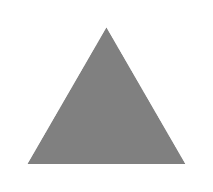
\begin{tikzpicture}
            \fill[gray] (0,0) -- (1,1.73) -- (2,0) -- cycle;
        \end{tikzpicture}
       \item 
\begin{tikzpicture}
            \fill[gray] (0,0) -- (2.2,0) -- (1.85,1.5) -- (0.35,1.5) -- cycle; 
            
        \end{tikzpicture}
        \item  
\begin{tikzpicture}
            \fill[gray] (0,0) rectangle (2,2);
        \end{tikzpicture}
        
        
    \end{enumerate}
    \end{multicols}


    \end{center}

    \begin{multicols}{4}
    \begin{enumerate}
         \item 0.69
        \item 0.88
        \item 0.98
        \item 1.37
    
    \end{enumerate}
       
    \end{multicols}

    \item A pair of spur gears with module 5 $mm$ and a center distance of 450 $mm$ is used for a speed reduction of 5:1. The number of teeth on pinion is \underline{\hspace{2cm}} \hfill{[GATE 2014]}\\

   
    \item Consider a cantilever beam, having negligible mass and uniform flexural rigidity, with length 0.01 $m$. The frequency of vibration of the beam, with a 0.5 $kg$ mass attached at the free tip, is 100 $Hz$. The flexural rigidity (in N$\cdot$m$^2$) of the beam is \underline{\hspace{2cm}} \hfill{[GATE 2014]}\\

    \item An ideal water jet with volume flow rate of 0.05 m$^3$/s strikes a flat plate placed normal to its path and exerts a force of 1000 $N$. Considering the density of water as 1000 $kg/m$ $^3$, the diameter (in $mm$) of the water jet is \underline{\hspace{2cm}} \hfill{[GATE 2014]}\\
 

    \item A block weighing 200 $N$ is in contact with a level plane whose coefficients of static and kinetic friction are 0.4 and 0.2, respectively. The block is acted upon by a horizontal force (in newton) $P = 10t$, where $t$ denotes the time in seconds. The velocity (in $m/s$) of the block attained after 10 seconds is \underline{\hspace{2cm}} \hfill{[GATE 2014]}\\

      \item A slider crank mechanism has slider mass of 10 $kg$, stroke of 0.2 $m$ and rotates with a uniform angular velocity of 10 $rad/s$. The primary inertia forces of the slider are partially balanced by a revolving mass of 6 $kg$ at the crank, placed at a distance equal to crank radius. Neglect the mass of connecting rod and crank. When the crank angle (with respect to slider axis) is 30$\degree$, the unbalanced force (in newton) normal to the slider axis is\underline{\hspace{2cm}} \hfill{[GATE 2014]}
\\
 \item An offset slider-crank mechanism is shown in the figure at an instant. Conventionally, the Quick  Return Ratio (QRR) is considered to be greater than one. The value of QRR is 

 
\begin{centering}
  \begin{figure}[!ht]
\centering
\resizebox{0.3\textwidth}{!}{%
\begin{circuitikz}
\tikzstyle{every node}=[font=\large]
\draw [ line width=1.2pt](3.75,11.75) to[short] (3.75,6.75);
\draw [ line width=1.2pt](3.75,6.75) to[short] (8.75,6.75);
\draw [ line width=1.2pt](8.75,11.75) to[short] (8.75,6.75);
\draw [ line width=1.2pt](3.75,11.75) to[short] (8.75,11.75);
\draw [line width=1.2pt, dashed] (5,11.75) -- (5,6.75);
\draw [line width=1.2pt, dashed] (7.5,11.75) -- (7.5,6.75);
\draw [line width=1.2pt, dashed] (3.75,10.5) -- (8.75,10.5);
\draw [line width=1.2pt, dashed] (3.75,8) -- (8.75,8);
\draw [ line width=1.2pt](6.25,11.75) to[short] (6.25,6.75);
\draw [ line width=1.2pt](3.75,9.25) to[short] (8.75,9.25);
\node [font=\large] at (4.35,7.25) {$\ast$};
\node [font=\large] at (7,9.9) {$\ast$};
\node [font=\large] at (8.1,8.5) {$\ast$};
\node [font=\large] at (8.25,11) {$\triangle$};
\node [font=\large] at (7,7.35) {$\triangle$};
\node [font=\large] at (5.7,9.8) {$\circ$};
\node [font=\large] at (8.1,7.25) {$\circ$};
\node [font=\large] at (7,8.5) {$\square$};
\node [font=\large] at (5.7,11) {$?$};
\end{circuitikz}
}%

\end{figure}
   
\end{centering}\hfill{[GATE 2014]}
 \\

  
\item A rigid uniform rod $AB$ of length $L$ and mass $m$ is hinged at $C$ such that $AC = L/3$, $CB = 2L/3$. Ends $A$ and $B$ are supported by springs of spring constant $k$. The natural frequency of the system is given by \\


\begin{centering}
     \begin{center}
\resizebox{0.3\textwidth}{!}{%
\begin{circuitikz}
\tikzstyle{every node}=[font=\large]
\fill[lightgray] (6.25,8.75) -- (7.75,10.25) -- (6.25,11.75) --(4.5,10) --cycle;
\draw [black, line width=1.2pt](6.25,11.75) to[short] (6.25,8.75);
\draw [black, line width=1.2pt](6.25,11.75) to[short] (7.75,10.25);
\draw [black, line width=1.2pt](6.25,8.75) to[short] (7.75,10.25);
\draw [black, line width=1.2pt](6.25,11.75) to[short] (4.5,10);
\draw [black, line width=1.2pt](4.5,10) to[short] (6.25,8.75);
\draw [black, line width=1.2pt, dashed] (4.5,10) -- (6.55,10.3);
\draw [black, line width=1.2pt, dashed] (6.25,11.75) -- (6.55,10.3);
\draw [black, line width=1.2pt, dashed] (6.55,10.3) -- (7.75,10.25);



\end{circuitikz}
}%
\end{center}


\end{centering}    
   
\hfill{[GATE 2014]}
    \begin{multicols}{4}
    \begin{enumerate}
        \item $\sqrt{\frac{k}{2m}}$
        \item $\sqrt{\frac{k}{m}}$
        \item $\sqrt{\frac{2k}{m}}$
        \item $\sqrt{\frac{5k}{m}}$
    \end{enumerate}
    \end{multicols}
    \item A hydrodynamic journal bearing is subject to 2000 $N$ load at a rotational speed of 2000 rpm. Both bearing bore diameter and length are 40 $mm$. If radial clearance is 20 $\mu m$ and bearing is lubricated with an oil having viscosity 0.03 $Pa.s$, the Sommerfeld number of the bearing is \underline{\hspace{2cm}}\hfill{[GATE 2014]}
   \\
    

    \item A 200 $mm$ long, stress-free rod at room temperature is held between two immovable rigid walls. The temperature of the rod is uniformly raised by 250$\degree C$. If the Young's modulus and coefficient of thermal expansion are 200 $GPa$ and $1 \times 10^{-5}/ \degree C$, respectively, the magnitude of the longitudinal stress (in $MPa$) developed in the rod is \underline{\hspace{2cm}}\hfill{[GATE 2014]}
  \\
  
\item 1.5 kg of water is in saturated liquid state at 2 bar ($v_f = 0.001061$ m$^3 /kg$, $u_f = 504.0$ $kJ/kg$, $h_f = 505$ $kJ/kg$). Heat is added in a constant pressure process till the temperature of water reaches 400$\degree C$ ($v = 1.5493$ m$^3 /kg$, $u = 2967.0$ $kJ/kg$, $h = 3277.0$ /, $kJ/kg$). The heat added (in $kJ$) in the process is \underline{\hspace{2cm}}\hfill{[GATE 2014]}
 \\
    
 \item Consider one dimensional steady state heat conduction across a wall (as shown in figure below) of thickness $30 \ \text{mm}$ and thermal conductivity $15 \ \text{W/m.K}$. At $x = 0$, a constant heat flux, $q'' = 1 \times 10^5 \ \text{W/m}^2$ is applied. On the other side of the wall, heat is removed from the wall by convection with a fluid at $25^\circ \text{C}$ and heat transfer coefficient of $250 \ \text{W/m}^2\cdot\text{K}$. The temperature (in $^\circ \text{C}$), at $x = 0$ is \underline{\hspace{2cm}}\hfill{[GATE 2014]}

\begin{center}
  \begin{center}
\resizebox{0.7\textwidth}{!}{%
\begin{circuitikz}
\tikzstyle{every node}=[font=\LARGE]
\draw [->, >=Stealth] (2.5,10.5) -- (3.75,10.5);
\draw [->, >=Stealth] (2.5,10.125) -- (3.75,10.125);
\draw [->, >=Stealth] (2.5,9.75) -- (3.75,9.75);
\draw [->, >=Stealth] (10,10.5) -- (11.25,10.5);
\draw [->, >=Stealth] (10,10.125) -- (11.25,10.125);
\draw [->, >=Stealth] (10,9.75) -- (11.25,9.75);
\draw [short] (6.25,8.75) .. controls (2.75,11.75) and (4.75,12.5) .. (6.25,8.75);
\draw [short] (13.75,8.75) .. controls (10,14) and (13,12.25) .. (13.64,8.9);
\node [font=\LARGE] at (9.5,10.25) {U};
\node [font=\normalsize] at (1.5,8.25) {Trailing Edge With Finite Angle};
\node [font=\normalsize] at (9.5,8.25) {Trailing Edge With cusp};
\node [font=\LARGE] at (1.75,10.25) {U};
\end{circuitikz}
}%
\end{center}
    \end{center}

 
\end{enumerate}

\end{document}

